\documentclass{article}

\usepackage{color}
\usepackage{tikz}
\usepackage{float}
\usepackage{tabularx}
\usepackage{amsmath}
\usepackage{amssymb}
\usepackage{listings}
\usepackage{enumitem}
\usepackage{syntax}
\usepackage{csquotes}
\usepackage{pgfplots}
\usepackage{parskip}
\usepackage{fancyhdr}
\usepackage{vmargin}
%\usepackage[backend=biber]{biblatex}
%\addbibresource{references.bib}


\definecolor{dkgreen}{rgb}{0,0.6,0}
\definecolor{gray}{rgb}{0.5,0.5,0.5}
\definecolor{mauve}{rgb}{0.58,0,0.82}

% Plots
\usepackage{pgfplots}
\usepackage{pgfplotstable}
\pgfplotsset{filter discard warning=false}
\pgfplotsset{
    discard if/.style 2 args={
        x filter/.append code={
            \edef\tempa{\thisrow{#1}}
            \edef\tempb{#2}
            \ifx\tempa\tempb
                \def\pgfmathresult{inf}
            \fi
        }
    },
    discard if not/.style 2 args={
        x filter/.append code={
            \edef\tempa{\thisrow{#1}}
            \edef\tempb{#2}
            \ifx\tempa\tempb
            \else
                \def\pgfmathresult{inf}
            \fi
        }
    },
    discard if smaller/.style n args={2}{
    	x filter/.code={
            \edef\tempa{\thisrow{#1}}
            \edef\tempb{#2}
                \ifnum\tempa<\tempb
                    \def\pgfmathresult{inf}
                \else
                \fi
        }
    },
    discard if larger/.style n args={2}{
    	x filter/.code={
            \edef\tempa{\thisrow{#1}}
            \edef\tempb{#2}
                \ifnum\tempa>\tempb
                    \def\pgfmathresult{inf}
                \else
                \fi
        }
    }
}


% Listings
\usepackage{algorithm}
\usepackage[noend]{algpseudocode}

\lstset{frame=tb,
  numbers=left,
  stepnumber=1,
  language=Java,
  aboveskip=3mm,
  belowskip=3mm,
  showstringspaces=false,
  columns=flexible,
  basicstyle={\small\ttfamily},
  numberstyle=\color{gray},
  keywordstyle=\color{blue},
  commentstyle=\color{dkgreen},
  stringstyle=\color{mauve},
  breaklines=true,
  breakatwhitespace=true,
  tabsize=2,
  moredelim=**[is][\color{red}]{@}{@},
}

\setlength{\grammarindent}{12em}

%\renewcommand{\lstlistingname}{Algorithm}
%\newcommand{\tablerow}[4]{ #1 & #2 & #3 & #4\\}
\newcommand{\n}[0]{\\[\baselineskip]}

% TITLE PAGE
% #1 - Module code
% #2 - Lecturer
\newcommand{\maketitlepage}[2]{
\begin{titlepage}
	\centering
    
\includegraphics[scale = 0.4]{imgs/logo.png}\\	% University Logo
	\textsc{\LARGE #1}\\[0.5 cm]				% Course Code
	\rule{\linewidth}{0.2 mm} \\[0.4 cm]
	{ \huge \bfseries \thetitle}
	\rule{\linewidth}{0.2 mm} \\[0.5 cm]
	\textsc{\large \thedate}\\[1.5 cm]
	
	\begin{minipage}{0.4\textwidth}
		\begin{flushleft} \large
			\emph{Lecturer:}\\
			#2
			\end{flushleft}
			\end{minipage}~
			\begin{minipage}{0.4\textwidth}
            
			\begin{flushright} \large
			\emph{Submitted By:} \\
			\theauthor
		\end{flushright}
        
	\end{minipage}\\[2 cm]
	
\end{titlepage}
}




\title{Classification of object colour using optical spectroscopy}
\author{140011146}

\makeatletter
\let\thetitle\@title
\let\theauthor\@author
\let\thedate\@date
\makeatother

\begin{document}

\maketitlepage{CS5014 Machine Learning}{David Harris-Birtill\\Kasim Terzi\'{c}}



\section{Introduction}

In this practical, two classification tasks were performed on an experimental dataset. 

\section{Binary Classification}

\subsection{Preprocessing}
Before any preprocessing is done, the data was split into training and test datasets. This is to ensure no bias when looking at the data, even for visualisations. The split is also stratified over the output to ensure the training and test sets have the same proportion of classes that is found in the original data. This again is done to prevent bias and overfitting as much as possible so that the trained model is not overfit to a subset of the data with a different proportion of classes. 
\n
Nothing was done about the negative intensities found in the data as this came from issues during data collection where the distance of the spectrometer changed. It is not trivial to account for the errors as the distance moved is not known. Further, scaling to the negative values to keep the intensities going from 0-100\% is likely to skew the data in an unknown way. Removing all data points where negative values exist would also hurt as the dataset is already quite small. TODO. Because of these reasons, the data was not cleaned for negative intensities. 


\subsubsection{Data visualisation}
First, the spectroscopy data can be visualised by plotting the intensities and wavelengths to see if there are visual patterns than can be seen in the data. As there are over nine hundred input features, it is likely many of them are either redundant or not well correlated to the input data. 

\begin{figure}[H]
\centering
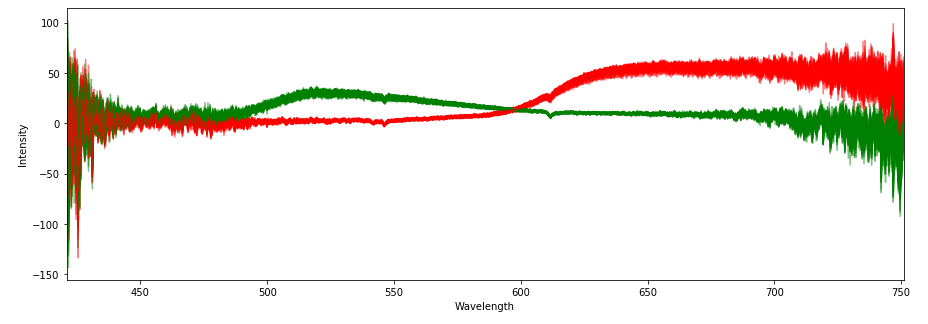
\includegraphics[width=1\textwidth, keepaspectratio]{imgs/binary-visual.png}
\caption{Initial plot of the data, showing the intensity of the wavelengths measured. The plot is colour coded with the output so any differences between the red and green data can be easily seen.}
\label{fig:binary-visual}
\end{figure}
\noindent
From the visualisation, it is interesting to see that for many wavelengths, there is a very clear distinction between the red and green intensities. This suggests that for those wavelengths, it would be very simple to classify. Further, the visualisation was created from all the training data, so it can be seen there are no large errors in the middle wavelengths where no data points incurred significant differences, which shows the consistency of the data. It can be see towards the start and end of the spectrum, the intensities are more varied, indicating possible errors during measurement. As such, it would make sense when choosing input features to mostly include features from the middle wavelengths where less possible errors occurred. 

\subsubsection{Data correlation}
Next, the correlation of each input feature wavelength can be calculated and plotted to see how the set of input features is correlated to the output. It is not feasible to plot each input feature's correlation separately due to the large number of features. Therefore all the features are put onto the same graph for comparison.
\begin{figure}[H]
\centering
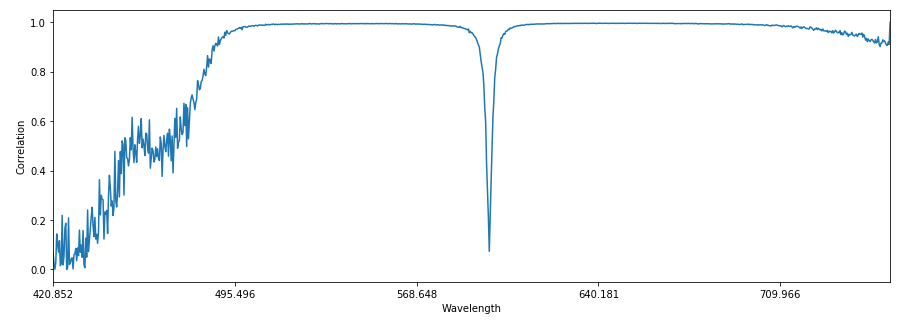
\includegraphics[width=1\textwidth, keepaspectratio]{imgs/binary-correlation.png}
\caption{Correlation of each wavelength input feature to the output classification.}
\label{fig:binary-correlation}
\end{figure}
\noindent
The curve of input feature correlation corresponds very closely to figure \ref{fig:binary-visual}. At the beginning where there seems to be more noise, the correlation is low. At the wavelengths where the red and green curves start to become distinct from each other, the correlation of that wavelength to the output class tends to perfect correlation. At the center where the red and green curves cross over, a dip in the correlation can be seen as it becomes difficult to distinguish the two in the overlap. This is good news and expected, as the clear difference between the red and green curves corresponds to a clear classification. 
\n
To show this more clearly, the histograms of a single input feature can be visualised.

\begin{figure}[H]
\centering
\subfigureimage{0.45\textwidth}
{imgs/binary-onefeaturebad.png}
{Histogram of a wavelength where there is high overlap and low correlation between the red and green curves.}
\hspace*{\fill}
\subfigureimage
{0.45\textwidth}
{imgs/binary-onefeaturegood.png}
{Histogram of a wavelength where the red and green curves are distinct and there is perfect correlation with the output class.}

\caption{Comparison of histograms of a single wavelength measurement. One taken at a low correlation wavelength and the other at a high correlation wavelength.}
\label{fig:binary-histogram-comparison}
\end{figure}
\noindent
The histograms in figure \ref{fig:binary-histogram-comparison} show the difference between an input feature with low correlation and an input feature with high correlation. The two wavelengths were arbitrarily chosen based on the correlation graph, but an obvious difference can still be seen. With low correlation, there is a lot of overlap between the two classes, which could also have been seen in figure \ref{fig:binary-visual}. For  the input feature with high correlation, the histogram shows very clearly the separation between the two classes. Figure \ref{fig:binary-histogram-more} further supports the fact that all input feature wavelengths where the correlation is high and a clear distinction seen in figure \ref{fig:binary-visual} have clear, separate intensities. As the histograms contain all data points from the split training set, it is very likely that a single input feature can lead to a high classification rate. 

\begin{figure}[H]
\subfigureimage{0.31\textwidth}
{imgs/binary-onefeature1.png}
{Wavelength 495.496}
\hspace*{\fill}
\subfigureimage{0.31\textwidth}
{imgs/binary-onefeature2.png}
{Wavelength 640.181}
\hspace*{\fill}
\subfigureimage{0.31\textwidth}
{imgs/binary-onefeature3.png}
{Wavelength 709.966}
\caption{Further histograms of highly correlated wavelengths, showing the separation of the two classes occurs for many different input features.}
\label{fig:binary-histogram-more}
\end{figure}



\subsection{Results}
From the preprocessing stage, it was shown that there are multiple input features where a clear distinction using just that single input feature could be seen between the two classes. As such, a single input feature is tried first for training to see what classification rates could be obtained. 
\begin{table}[H]
\centering
\begin{tabular}{| c | c |}
\hline
\textbf{Input feature} & \textbf{Accuracy} \\
\hline
Wavelength 421.228 & 0.5 \\
\hline
Wavelength 495.496 & 1.0 \\
\hline
Wavelength 568.648 & 1.0 \\
\hline
Wavelength 640.181 & 1.0 \\
\hline
Wavelength 709.966 & 1.0 \\
\hline
\end{tabular}
\caption{Results of training a logistic regression model on a single input feature.}
\end{table}
\noindent
Despite the indications that the data would be easy to classify, the predictions from the logistic regression model are suspiciously high. All single input features used that had a high correlation gave perfect accuracy during prediction. The first thought was that perhaps the model is overfitting, so the same training is done again with k-fold cross validation. 
\begin{table}[H]
\centering
\begin{tabular}{| c | c | c | c |}
\hline
\textbf{Input feature} & \textbf{5 fold accuracy} & \textbf{10 fold accuracy} & \textbf{25 fold accuracy} \\
\hline
Wavelength 421.228 & 0.5 & 0.49 & 0.5 \\
\hline
Wavelength 495.496 & 1.0 & 1.0 & 1.0 \\
\hline
Wavelength 568.648 & 1.0 & 1.0 & 1.0 \\
\hline
Wavelength 640.181 & 1.0 & 1.0 & 1.0 \\
\hline
Wavelength 709.966 & 1.0 & 1.0 & 1.0 \\
\hline
\end{tabular}
\caption{Accuracy of using k-fold cross validation to show the logistic regression model is not overfitting.}
\end{table}
\noindent
Even with using a high k-fold cross validation, the strong input features continued to get 100\% accuracy, showing it is unlikely due to overfitting but because the data and those specific input features lends themselves well to a binary classification. It was further confirmed how well defined the classification was by splitting the training data into an even smaller dataset with only 10\% of the training dataset used for training and testing on the rest of the training data. Here there is a slight discrepancy between  training and testing accuracy where certain input features obtained slightly lower accuracy when running on the test data. This tells us that even with a very well defined classes as seen from previous training models and visualisations, it is difficult for models to generalise well given very few samples. At the same time, the fact that such a high testing accuracy could still be obtained from such a low number of training samples once again shows the clear difference between the classes.

\begin{table}[H]
\centering
\begin{tabular}{| c | c | c |}
\hline
\textbf{Input feature} & \textbf{Training accuracy} & \textbf{Testing accuracy}\\
\hline
Wavelength 421.228 & 0.67 & 0.46\\
\hline
Wavelength 495.496 & 1.0 & 0.98\\
\hline
Wavelength 568.648 & 1.0 & 0.99\\
\hline
Wavelength 640.181 & 1.0 & 1.0\\
\hline
Wavelength 709.966 & 1.0 & 1.0\\
\hline
\end{tabular}
\caption{Accuracy of training logistic regression on 10\% of the training data and testing on the remaining 90\%.}
\end{table}
Two more approaches were used as a final way of checking that one input feature is enough for a good classification of this problem. First the accuracies of each single input feature is calculated by training a logistic regression model with that feature and plotting the accuracies. Finally, recursive feature elimination was used to get the accuracy score as the number of features used increased to show any more than two input features will always give 100\% accuracy. 
\begin{figure}[H]
\centering
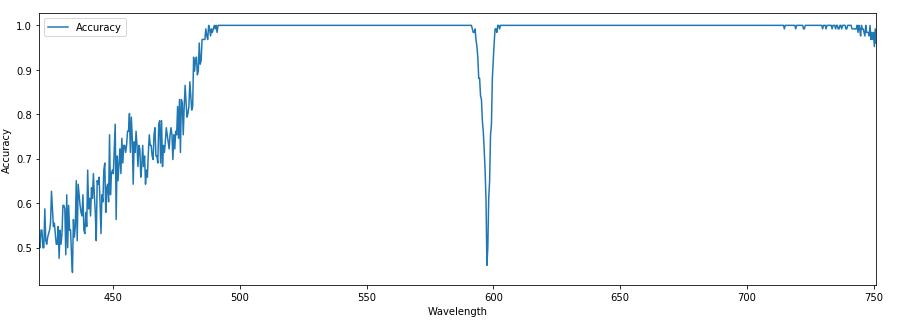
\includegraphics[width=1\textwidth]{imgs/binary-accuracy.png}
\caption{All input feature wavelengths trained individually and their accuracies graphed.}
\label{fig:binary-accuracy}
\end{figure}
%
\begin{figure}[H]
\centering
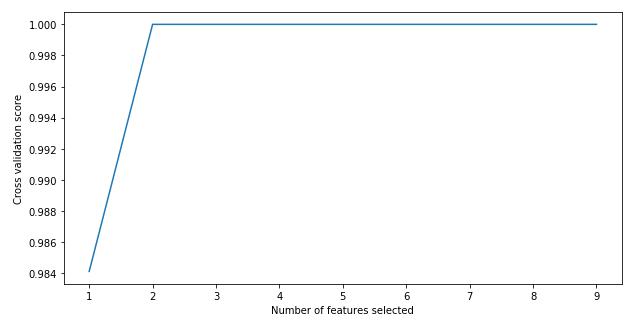
\includegraphics[width=1\textwidth, keepaspectratio]{imgs/binary-numfeatures.png}
\caption{Cross validation accuracy score of increasing number of features using recursive feature elimination.}
\label{fig:binary-accuracyrfecv}
\end{figure}
\noindent
Figure \ref{fig:binary-accuracy} shows the accuracy of each input feature when used alone to train the logistic regression model. It can be seen to be very similar to figure \ref{fig:binary-correlation} which showed the correlation of each input feature. This indicates the well correlated features are also the ones that have good accuracies with little noise disrupting this pattern. The graph of accuracy obtain from recursive feature elimination with cross validation does not confirm it is always the case the one input feature is enough for perfect classification. This is because of the wavelengths at the beginning and end of the data where there is more overlap. However, one input feature already gets a 0.992 classification rate on average and any more than one feature always gets 100\%. 

\subsection{Evaluation}
From the initial visualisations of the binary classification data, it could be seen that for a range of wavelengths, the two classes of red and green colours were easily distinguishable by eye. This was further confirmed by graphing the correlation of each wavelength to the output classification and shown clearly by plotting the histogram of a single wavelength, which showed a clear separation between the classes. Because of these observations, it was not a huge surprise that a simple logistic regression model was able to perform perfect classification on the training data, using specific single input features. The results were confirmed to not be due to overfitting, as k-fold validation was performed with a large value of k. Moreover, it was shown that with a training set size of just 10\% (12 data points), the high classification rate was still retained when predicting the other 90\% (114 data points).
\n
The results make sense when coming back to what the actual classification problem is. The data represents spectroscopy data with red and green colours placed under the device. As red and green are very distinct colours with different wavelengths, it was natural that there would be a clear separation between the colours.
\n
Finally, the use of a single feature obtaining such a high classification rate was confirmed with the use of recursive feature elimination with cross validation. This shows how the accuracy score improves as the number of features used increases.

At one 
The fact that this classification problem could be easily solved with the simplest logistic regression model using only one input feature and a minuscule number of training samples shows TODO. 
\section{Multiclass Classification}
For the multiclass classification, many of the same steps as the binary task were taken. Because of the added complexity of more classes, the results were not the same and hence the steps deviate from the binary task at a certain point. 

\subsection{Preprocessing}

\subsubsection{Data visualisation}

\begin{figure}[H]
\centering
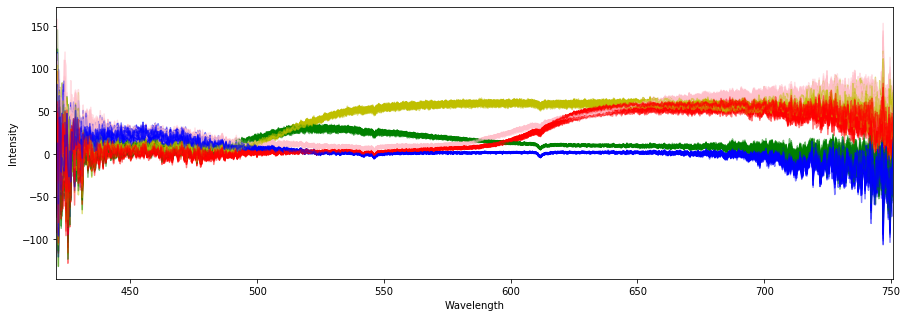
\includegraphics[width=1\textwidth, keepaspectratio]{imgs/multiclass-visual.png}
\caption{Plot of the data to show the intensity of wavelengths of the different colour classes.}
\end{figure}

\subsubsection{Data correlation}

\begin{figure}[H]
\centering
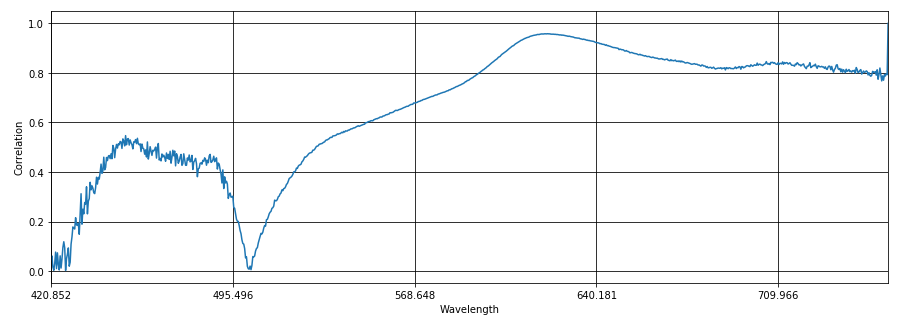
\includegraphics[width=1\textwidth, keepaspectratio]{imgs/multiclass-correlation.png}
\caption{Correlation of each wavelength input feature to the colour classification.}
\end{figure}

\subsection{Results}

\section{Conclusion and Evaluation}

%\printbibliography

\end{document}



